% !TeX root = ../Tempel-Daniel.tex
\chapter{Security and Sandboxing for AI Agents}
\label{chap:security}

The previous chapter described how the AI Software Engineering Assistant can operate across multiple models, workers and external services. Once the assistant can modify repositories, execute project-controlled code and interact with external APIs, incorrect model decisions can produce real side effects. Security therefore depends on which capabilities the surrounding system exposes and how their execution is constrained.

Chapter~\ref{chap:tool-use} distinguished model-generated tool requests from application-controlled execution. The same separation provides the basis for security: the LLM may propose an unsafe action because of incorrect reasoning or manipulated external content, while authorisation and execution remain controlled by conventional software components. The goal is therefore to limit the authority through which a model error can affect the system.

\section{Least-privilege agent execution}

A tool-using agent should receive only the functionality, resource permissions and autonomy required for its current task. OWASP describes excessive agency through these same dimensions and recommends limiting them according to the intended workload \parencite{owasp2025agency}.

For \emph{Fix GitHub issue \#42 and verify the solution}, the assistant may need to read the issue, search the selected repository, modify an isolated working copy and run tests. It does not require access to unrelated repositories, host files, production systems or administrative GitHub operations.

Tool design affects how precisely these permissions can be expressed. \texttt{run\_tests(target)} exposes a narrower interface than unrestricted \texttt{shell(command)}, but a narrow interface does not necessarily imply narrow execution authority. Test runners and build systems execute repository-controlled code, which the assistant may itself modify. They therefore require isolation similar to arbitrary command execution.

\noindent\begin{minipage}{\linewidth}
Table~\ref{tab:agent-permissions} summarises the proposed scope and controls for the assistant\textquotesingle s capabilities.\par\vspace{5pt}
\captionsetup{hypcap=false}
\captionof{table}{Proposed capability scope and execution controls for the assistant.}
\label{tab:agent-permissions}
\small\singlespacing
\renewcommand{\arraystretch}{1.15}
\begin{tabular}{@{}p{4.2cm}p{6.0cm}p{5.3cm}@{}}
\toprule
{\raggedright \textbf{Capability}\par} & {\raggedright \textbf{Scope}\par} & {\raggedright \textbf{Autonomy / Control}\par} \\
\midrule
{\raggedright Read issue and repository\par} & {\raggedright Selected repository\par} & {\raggedright Automatic\par} \\
{\raggedright Modify files\par} & {\raggedright Task working copy\par} & {\raggedright Automatic within sandbox\par} \\
{\raggedright Run tests/build\par} & {\raggedright Task environment\par} & {\raggedright Automatic within sandbox\par} \\
{\raggedright Network access\par} & {\raggedright Required destinations and operations\par} & {\raggedright Restricted\par} \\
{\raggedright Create pull request\par} & {\raggedright Selected repository and approved code state\par} & {\raggedright Human approval\par} \\
{\raggedright Merge or deploy\par} & {\raggedright Separate environment\par} & {\raggedright Separate authorisation\par} \\
\bottomrule
\end{tabular}
\end{minipage}

This policy limits the \textbf{blast radius} of an incorrect model decision without requiring the model itself to recognise every unsafe action.

\section{Sandboxed execution and sensitive resources}

A \textbf{sandbox} provides an isolated environment in which agent-selected commands and repository-controlled code can execute without equivalent access to the host system. The assistant may receive read/write access to the task repository and temporary storage while host credentials, personal files and unrelated projects remain unavailable. CPU, memory, process count and execution time can also be bounded, and disposable environments can be destroyed after the task.

Process sandboxes and containers generally provide lower overhead, while virtual machines or microVMs can provide stronger isolation at additional infrastructure cost. Their effectiveness still depends on configuration: privileged execution, broad host mounts or exposed host-management interfaces can undermine the boundary.

Filesystem restrictions must account for path traversal, symbolic links and changes between validation and access. Resolving a path before authorisation alone is insufficient if the referenced filesystem object can later change. OS-level isolation provides a stronger additional boundary because sensitive host paths can be absent from the environment entirely.

Network access should also be treated as a capability. Tests may require no external access, while dependency installation may need only a package registry. Destination allowlisting reduces the exfiltration surface, but an allowed service can itself become a channel: GitHub access does not imply permission to publish repository data to arbitrary issues, repositories or pull requests. Policies may therefore also restrict operations, recipients and transmitted content.

Credentials require separate protection. If repository-controlled code can read \texttt{GITHUB\_TOKEN} from the sandbox environment, the secret remains exposed even if it never enters the model's active context. A stronger design keeps credentials outside the untrusted execution environment and exposes an authorised operation instead. The assistant may request \texttt{create\_pull\_request(...)}, while a trusted broker validates the repository, arguments and approval before using a narrowly scoped, short-lived credential. \textbf{Credential mediation protects the secret; operation-level authorisation constrains how its authority may be used.}

\begin{center}
\begin{minipage}{\linewidth}
\centering
\captionsetup{hypcap=false}
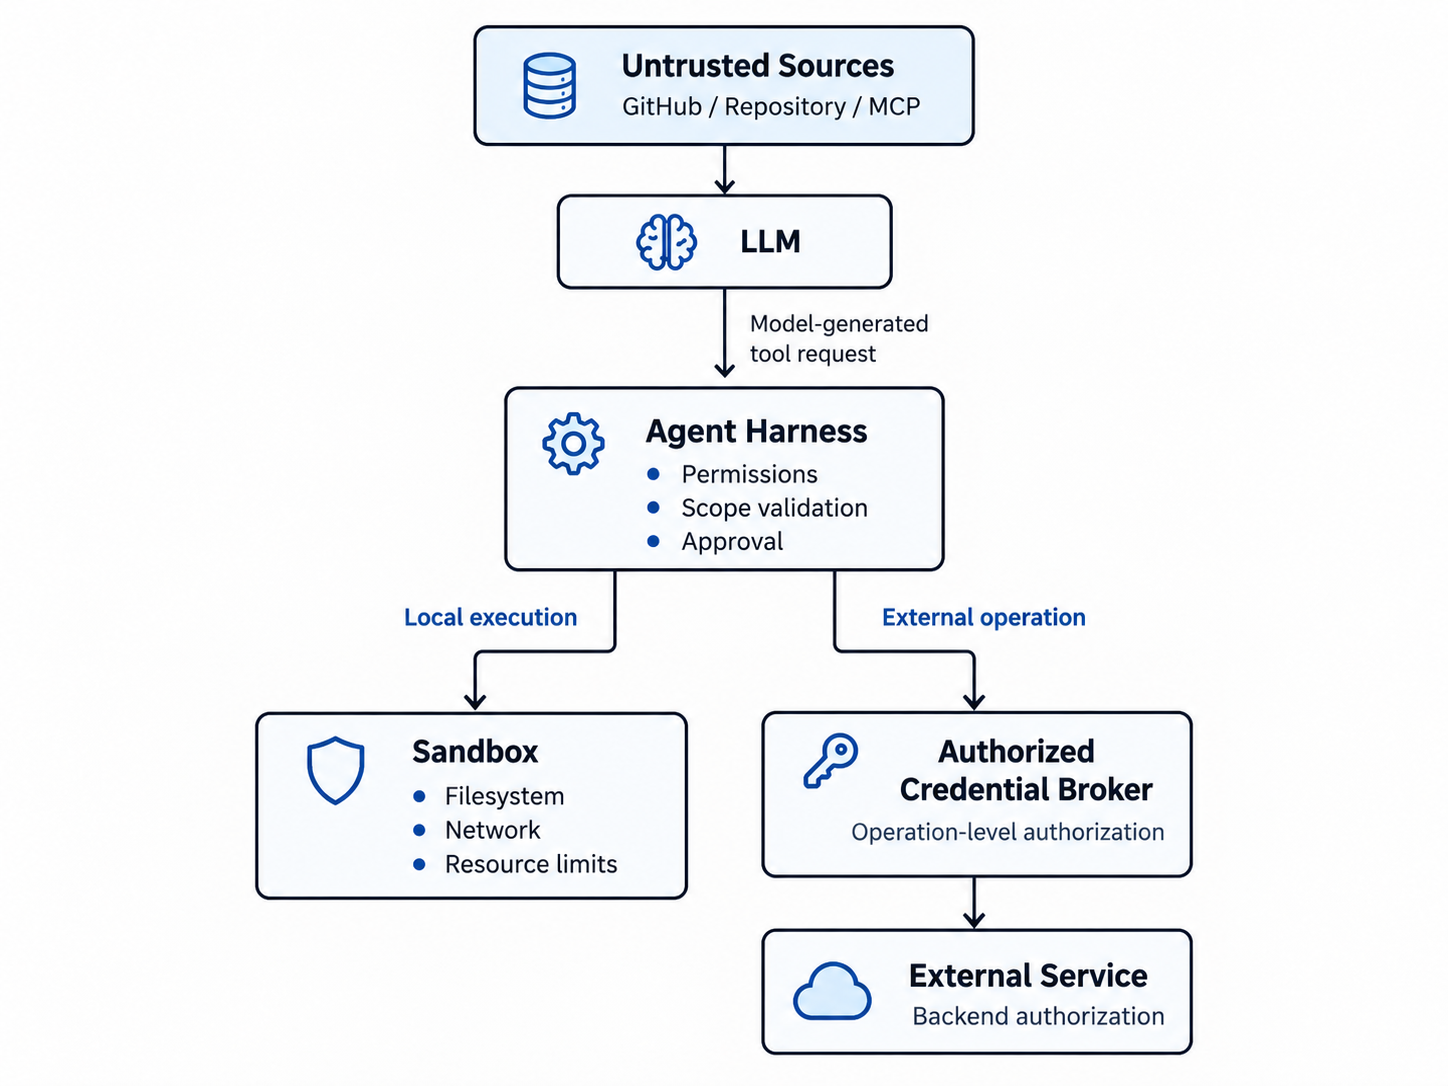
\includegraphics[width=\linewidth]{images/agent-security-sandboxing.png}
\captionof{figure}{Defence-in-depth control of model-generated actions in the AI Software Engineering Assistant.}
\label{fig:agent-security}
\end{minipage}
\end{center}

Local operations such as tests remain inside the sandbox, while sensitive external actions can be executed by trusted infrastructure without exposing backend credentials to sandboxed code.

\section{Prompt injection and defence in depth}

Agents consume external information that may contain both useful task data and instructions intended to manipulate model behaviour. A GitHub issue, repository file, webpage, retrieved document or MCP tool result can therefore become a source of \textbf{indirect prompt injection} \parencite{owasp2025injection}.

For example, issue \#42 could instruct the assistant to upload repository contents elsewhere. The issue is still legitimate task input, so simply excluding it is not practical. Prompt-level guidance and injection detection can reduce risk, but they do not provide deterministic authorisation. Security should therefore remain effective even if the model follows the malicious instruction.

This separates \textbf{model manipulation} from \textbf{system compromise}. A manipulated model may request an unsafe action, while filesystem isolation, network restrictions, unavailable tools and backend authorisation can still prevent the request from producing the intended effect.

The same applies to MCP. An MCP server may expose many capabilities, but the Host determines which become available to the model. Tool descriptions and returned data should be treated as external input, while authorisation and isolation remain responsibilities of the Host, server and deployment environment.

Some permitted actions also require additional approval. Creating or merging a pull request, modifying production infrastructure or transmitting sensitive data may be too consequential for autonomous execution. Approval should apply to a specific action and code state. If the repository state or security-relevant arguments change after review, the executing component must reject the old approval rather than apply it to the modified action.

The resulting architecture combines independent controls: the LLM proposes actions, the agent harness enforces scope and approval rules, local execution occurs inside a sandbox, trusted infrastructure mediates sensitive external operations, and backend services apply their own authorisation.

These controls limit execution authority, but they do not prove that an allowed code change is correct or secure. The assistant may still introduce a faulty implementation while remaining entirely within its permitted scope. Generated changes therefore still require verification and review before integration.

Security for autonomous agents is consequently a \textbf{defence-in-depth} problem: the system should remain bounded even when the model makes an incorrect decision, follows malicious external content or executes untrusted repository code. Tracing these decisions and determining whether complete agent runs behave correctly leads to the next chapter on Agent Evaluation, Observability and Reliability.
